% This is the Reed College LaTeX thesis template. Most of the work
% for the document class was done by Sam Noble (SN), as well as this
% template. Later comments etc. by Ben Salzberg (BTS). Additional
% restructuring and APA support by Jess Youngberg (JY).
% Your comments and suggestions are more than welcome; please email
% them to cus@reed.edu
%
% See http://web.reed.edu/cis/help/latex.html for help. There are a
% great bunch of help pages there, with notes on
% getting started, bibtex, etc. Go there and read it if you're not
% already familiar with LaTeX.
%
% Any line that starts with a percent symbol is a comment.
% They won't show up in the document, and are useful for notes
% to yourself and explaining commands.
% Commenting also removes a line from the document;
% very handy for troubleshooting problems. -BTS

% As far as I know, this follows the requirements laid out in
% the 2002-2003 Senior Handbook. Ask a librarian to check the
% document before binding. -SN

%%
%% Preamble
%%
% \documentclass{<something>} must begin each LaTeX document
\documentclass[12pt,twoside]{reedthesis}
% Packages are extensions to the basic LaTeX functions. Whatever you
% want to typeset, there is probably a package out there for it.
% Chemistry (chemtex), screenplays, you name it.
% Check out CTAN to see: http://www.ctan.org/
%%
\usepackage{graphicx,latexsym}
\usepackage{amsmath}
\usepackage{amssymb,amsthm}
\usepackage{longtable,booktabs,setspace}
\usepackage{chemarr} %% Useful for one reaction arrow, useless if you're not a chem major
\usepackage[hyphens]{url}
% Added by CII
\usepackage{hyperref}
\usepackage{lmodern}
\usepackage{float}
\floatplacement{figure}{H}
% End of CII addition
\usepackage{rotating}

% Next line commented out by CII
%%% \usepackage{natbib}
% Comment out the natbib line above and uncomment the following two lines to use the new
% biblatex-chicago style, for Chicago A. Also make some changes at the end where the
% bibliography is included.
%\usepackage{biblatex-chicago}
%\bibliography{thesis}


% Added by CII (Thanks, Hadley!)
% Use ref for internal links
\renewcommand{\hyperref}[2][???]{\autoref{#1}}
\def\chapterautorefname{Chapter}
\def\sectionautorefname{Section}
\def\subsectionautorefname{Subsection}
% End of CII addition

% Added by CII
\usepackage{caption}
\captionsetup{width=5in}
% End of CII addition

% \usepackage{times} % other fonts are available like times, bookman, charter, palatino

% Syntax highlighting #22

% To pass between YAML and LaTeX the dollar signs are added by CII
\title{Proto-Solutrean lithic technology of Western Iberia: sites of Vale Boi and Lapa do Picareiro}
\author{Joana Belmiro}
% The month and year that you submit your FINAL draft TO THE LIBRARY (May or December)
\date{May 2020}
\division{Faculdade de Ciências Humanas e Sociais}
\advisor{João Cascalheira}
\institution{Universidade do Algarve}
\degree{Mestrado em Arqueologia}
%If you have two advisors for some reason, you can use the following
% Uncommented out by CII
% End of CII addition

%%% Remember to use the correct department!
\department{Arqueologia}
% if you're writing a thesis in an interdisciplinary major,
% uncomment the line below and change the text as appropriate.
% check the Senior Handbook if unsure.
%\thedivisionof{The Established Interdisciplinary Committee for}
% if you want the approval page to say "Approved for the Committee",
% uncomment the next line
%\approvedforthe{Committee}

% Added by CII
%%% Copied from knitr
%% maxwidth is the original width if it's less than linewidth
%% otherwise use linewidth (to make sure the graphics do not exceed the margin)
\makeatletter
\def\maxwidth{ %
  \ifdim\Gin@nat@width>\linewidth
    \linewidth
  \else
    \Gin@nat@width
  \fi
}
\makeatother

\renewcommand{\contentsname}{Table of Contents}
% End of CII addition

\setlength{\parskip}{0pt}

% Added by CII

\providecommand{\tightlist}{%
  \setlength{\itemsep}{0pt}\setlength{\parskip}{0pt}}

\Acknowledgements{

}

\Dedication{

}

\Preface{

}

\Abstract{
The present study aims to answer the question: what impact did the Heinrich 2 event have on the technological organization of human communities, at the onset of the last glacial maximum, in south western Iberia? The impact of this event on the Gravettian-Soluttrean transition has been previously suggested (Bradtmöller, Pastoors, Weninger, \& Weniger, 2012). However, the existing models do not consider the Proto-Solutrean technocomplex as an individual phase for this transition (Cascalheira \& Bicho, 2013).

\par

To address this question, this study analysed the lithic assemblages from Vale Boi (south Portugal) and Lapa do Picareiro (central Portugal). We aimed to understand the technological patterns and raw material exploitation during the Proto-Solutrean, and test the existing models with assemblages from recently excavated sites, while expanding the geographic range.

The analysis followed a technologic and morphologic attribute approach. The retrieved data was then analysed through descritive statistics in R environment.

Results show the existence of two occupations within the assemblages. The first, with high frequency of quartz use for bladelet production, seems to reflect a Terminal Gravettian horizon. The appearance of Vale Comprido technology and lower quartz frequencies in a second moment in Vale Boi seem to represent a Proto-Solutrean occupation. The second horizon in Lapa do Picareiro, with the presence of Vale Comprido-like technology but with low flattening ratios may be attributed to a Proto-Solutrean or an Early Solutrean occupation.

The Terminal Gravettian and Proto-Solutrean seem to be chronologically different phases, in concordance with the Three-Phase model for the Proto-Solutrean (Zilhão, 1997). The similarities between Vale Boi and the Estremadura may be explained by the expansion of social networks (Cascalheira \& Bicho, 2013). Associated with the dominance of different technologic patterns and intensive use of quartz, we may understand these horizons as a moment of cultural reorganization, onset by environmental pressures.

Keywords: Upper Paleolithic; Attribute analysis; Raw material exploitation; Climatic changes.
}

\Resumo{
O objetivo desta tese é responder à seguinte pergunta: que impacto teve o evento climático Heinrich 2 (HE 2) na organização tecnológica das comunidades de caçadores-recolectores no início do último máximo glacial (LGM), no sudoeste peninsular?

\par

Esta questão está intimamente ligada ao entendimento de certos eventos climáticos abruptos, tais como os eventos de Heinrich ou os Estados Glaciares, com a substituição de culturas ao longo do Paleolítico Superior. Um destes momentos de substituição correlaciona a passagem do Gravetense para o Solutrense com o evento HE 2 e com o Estádio Glacial 3, possivelmente sobreposta pelo LGM. Neste paradigma, as mudanças climáticas desencadeiam mudanças sociais, através do colapso de tradições que depois são reorganizadas, de forma a corresponder às novas condições ambientais e paisagísticas. No entanto, nos modelos existentes, o Proto-Solutrense não surge como um tecnocomplexo individualizado, existindo assim uma lacuna no entendimento atual do processo de transição entre os dois horizontes culturais supramencionados.

O Proto-Solutrense, representado sobretudo na Estremadura Portuguesa, é entendido como um tecnocomplexo de transição, ocorrendo entre os 26 000 cal BP e 25 400 cal BP, e caracterizado por mudanças na tecnologia e preferência de matérias-primas, existindo dois modelos para a sua evolução: modelo em duas etapas; e modelo em três etapas.

O modelo em duas etapas considera a existência do Gravetense Final e Proto-Solutrense, caracterizado pelo uso intensivo de quartzo e estratégias de produção para obtenção de lamelas em núcleos carenados e obtenção de suportes convergentes para pontas de Vale Comprido, sendo, no entanto, caracterizado por uma alta variabilidade interna. O modelo em três etapas consiste na evolução do Gravetense Final para uma etapa intermédia (no modelo das duas etapas considerada uma fácies funcional do Proto-Solutrense), caracterizada pelo uso intensivo do quartzo, estratégias de redução para obtenção de lamelas em núcleos carenados, seguida de uma fase Proto-Solutrense caracterizada pela diminuição do uso do quartzo e estratégias de redução para obtenção de suportes convergentes para pontas de Vale Comprido.
O conhecimento atual do Proto-Solutrense apresenta-se truncado, no entanto, pela antiguidade de algumas escavações e a sua restrição geográfica à Estremadura Portuguesa.

De forma a responder à questão supramencionada, assim como contribuir para o conhecimento do Proto-Solutrense no sudoeste Peninsular, foram analisados os conjuntos líticos de Vale Boi (sul de Portugal) e Lapa do Picareiro (Portugal central), ambos escavados nos últimos 20 anos com recurso a estações totais. Esta análise teve a finalidade de entender os padrões tecnológicos e de exploração do território durante o Proto-Solutrense, através dos seguintes objetivos: 1) entender e explicar os padrões tecnológicos e de preferência de matérias-primas intra-sítio; 2) estabelecer paralelos entre os dois sítios; 3) comparar estes resultados com os obtidos em outros sítios com conjuntos Proto-Solutrenses, sobretudo da Estremadura.

A análise seguiu uma abordagem de atributos tecnológicos e morfológicos, seguida de uma fase de tratamento estatístico através de duas metodologias: estatística descritiva e multivariada, ambas efetuadas em ambiente R. A análise multivariada segue a metodologia já descrita noutros trabalhos (Tostevin 2012; Scerri et al.~2014), e que passa pelo agrupamento de vários atributos em domínios tecnológicos, cada qual representando uma escolha do talhador(a) em alturas chave do talhe, de forma a reduzir a variabilidade interna dos conjuntos.

Palavras-chave: Paleolítico Superior; Padrões tecnológicos; Exploração de matérias-primas.
}

	\usepackage[T1]{fontenc}
\usepackage[utf8]{inputenc}
	\usepackage{booktabs}
\usepackage{longtable}
\usepackage{array}
\usepackage{multirow}
\usepackage{wrapfig}
\usepackage{float}
\usepackage{colortbl}
\usepackage{pdflscape}
\usepackage{tabu}
\usepackage{threeparttable}
\usepackage{threeparttablex}
\usepackage[normalem]{ulem}
\usepackage{makecell}
\usepackage{xcolor}
% End of CII addition
%%
%% End Preamble
%%
%
\begin{document}

% Everything below added by CII
  \maketitle

\frontmatter % this stuff will be roman-numbered
%\pagestyle{empty} % this removes page numbers from the frontmatter


  \begin{abstract}
    The present study aims to answer the question: what impact did the Heinrich 2 event have on the technological organization of human communities, at the onset of the last glacial maximum, in south western Iberia? The impact of this event on the Gravettian-Soluttrean transition has been previously suggested (Bradtmöller, Pastoors, Weninger, \& Weniger, 2012). However, the existing models do not consider the Proto-Solutrean technocomplex as an individual phase for this transition (Cascalheira \& Bicho, 2013).
    
    \par
    
    To address this question, this study analysed the lithic assemblages from Vale Boi (south Portugal) and Lapa do Picareiro (central Portugal). We aimed to understand the technological patterns and raw material exploitation during the Proto-Solutrean, and test the existing models with assemblages from recently excavated sites, while expanding the geographic range.
    
    The analysis followed a technologic and morphologic attribute approach. The retrieved data was then analysed through descritive statistics in R environment.
    
    Results show the existence of two occupations within the assemblages. The first, with high frequency of quartz use for bladelet production, seems to reflect a Terminal Gravettian horizon. The appearance of Vale Comprido technology and lower quartz frequencies in a second moment in Vale Boi seem to represent a Proto-Solutrean occupation. The second horizon in Lapa do Picareiro, with the presence of Vale Comprido-like technology but with low flattening ratios may be attributed to a Proto-Solutrean or an Early Solutrean occupation.
    
    The Terminal Gravettian and Proto-Solutrean seem to be chronologically different phases, in concordance with the Three-Phase model for the Proto-Solutrean (Zilhão, 1997). The similarities between Vale Boi and the Estremadura may be explained by the expansion of social networks (Cascalheira \& Bicho, 2013). Associated with the dominance of different technologic patterns and intensive use of quartz, we may understand these horizons as a moment of cultural reorganization, onset by environmental pressures.
    
    Keywords: Upper Paleolithic; Attribute analysis; Raw material exploitation; Climatic changes.
  \end{abstract}
  \begin{resumo}
    O objetivo desta tese é responder à seguinte pergunta: que impacto teve o evento climático Heinrich 2 (HE 2) na organização tecnológica das comunidades de caçadores-recolectores no início do último máximo glacial (LGM), no sudoeste peninsular?
    
    \par
    
    Esta questão está intimamente ligada ao entendimento de certos eventos climáticos abruptos, tais como os eventos de Heinrich ou os Estados Glaciares, com a substituição de culturas ao longo do Paleolítico Superior. Um destes momentos de substituição correlaciona a passagem do Gravetense para o Solutrense com o evento HE 2 e com o Estádio Glacial 3, possivelmente sobreposta pelo LGM. Neste paradigma, as mudanças climáticas desencadeiam mudanças sociais, através do colapso de tradições que depois são reorganizadas, de forma a corresponder às novas condições ambientais e paisagísticas. No entanto, nos modelos existentes, o Proto-Solutrense não surge como um tecnocomplexo individualizado, existindo assim uma lacuna no entendimento atual do processo de transição entre os dois horizontes culturais supramencionados.
    
    O Proto-Solutrense, representado sobretudo na Estremadura Portuguesa, é entendido como um tecnocomplexo de transição, ocorrendo entre os 26 000 cal BP e 25 400 cal BP, e caracterizado por mudanças na tecnologia e preferência de matérias-primas, existindo dois modelos para a sua evolução: modelo em duas etapas; e modelo em três etapas.
    
    O modelo em duas etapas considera a existência do Gravetense Final e Proto-Solutrense, caracterizado pelo uso intensivo de quartzo e estratégias de produção para obtenção de lamelas em núcleos carenados e obtenção de suportes convergentes para pontas de Vale Comprido, sendo, no entanto, caracterizado por uma alta variabilidade interna. O modelo em três etapas consiste na evolução do Gravetense Final para uma etapa intermédia (no modelo das duas etapas considerada uma fácies funcional do Proto-Solutrense), caracterizada pelo uso intensivo do quartzo, estratégias de redução para obtenção de lamelas em núcleos carenados, seguida de uma fase Proto-Solutrense caracterizada pela diminuição do uso do quartzo e estratégias de redução para obtenção de suportes convergentes para pontas de Vale Comprido.
    O conhecimento atual do Proto-Solutrense apresenta-se truncado, no entanto, pela antiguidade de algumas escavações e a sua restrição geográfica à Estremadura Portuguesa.
    
    De forma a responder à questão supramencionada, assim como contribuir para o conhecimento do Proto-Solutrense no sudoeste Peninsular, foram analisados os conjuntos líticos de Vale Boi (sul de Portugal) e Lapa do Picareiro (Portugal central), ambos escavados nos últimos 20 anos com recurso a estações totais. Esta análise teve a finalidade de entender os padrões tecnológicos e de exploração do território durante o Proto-Solutrense, através dos seguintes objetivos: 1) entender e explicar os padrões tecnológicos e de preferência de matérias-primas intra-sítio; 2) estabelecer paralelos entre os dois sítios; 3) comparar estes resultados com os obtidos em outros sítios com conjuntos Proto-Solutrenses, sobretudo da Estremadura.
    
    A análise seguiu uma abordagem de atributos tecnológicos e morfológicos, seguida de uma fase de tratamento estatístico através de duas metodologias: estatística descritiva e multivariada, ambas efetuadas em ambiente R. A análise multivariada segue a metodologia já descrita noutros trabalhos (Tostevin 2012; Scerri et al.~2014), e que passa pelo agrupamento de vários atributos em domínios tecnológicos, cada qual representando uma escolha do talhador(a) em alturas chave do talhe, de forma a reduzir a variabilidade interna dos conjuntos.
    
    Palavras-chave: Paleolítico Superior; Padrões tecnológicos; Exploração de matérias-primas.
  \end{resumo}
  \hypersetup{linkcolor=black}
  \setcounter{tocdepth}{2}
  \tableofcontents

  \listoftables

  \listoffigures


\mainmatter % here the regular arabic numbering starts
\pagestyle{fancyplain} % turns page numbering back on

\hypertarget{if-you-have-more-two-advisors-un-silence-line-7}{%
\chapter{If you have more two advisors, un-silence line 7}\label{if-you-have-more-two-advisors-un-silence-line-7}}

Placeholder

\hypertarget{introduction}{%
\chapter{Introduction}\label{introduction}}

The replacement of the Gravettian technocomplex by the Solutrean, impacted by adverse climatic conditions during the Heinrich Event 2 (HE2), continues to be an essential topic for understanding the Upper Paleolithic and Human adaptations to climatic changes. The Proto-Solutrean is, in this topic, an essential piece to understand how hunter-gatherer communities adapted, reinvented and destroyed their social and technologic organization which eventually allowed the development of the Solutrean. However, most of what is known for this technocomplex is still geographically constricted and lacking good chronological markers (Cascalheira \& Bicho, 2013), which hampers the understanding of the Proto-Solutrean itself and its role in the Gravettian-Solutrean transition.

By understanding the need to better comprehend the Proto-Solutrean and how adverse climate impacted these communities, this study aims to answer the following question: what impact did the HE 2 have on the technological organization of human communities, at the onset of the last glacial maximum, in south western Iberia? To do so, this study will analyse the lithic terminal gravettian/proto-solutrean assemblages of two recently excavated sites with resource to total stations, Vale Boi (south of Portugal) and Lapa do Picareiro (central Portugal).

To answer this question, we aim to accomplish the following goals:
\begin{itemize}
\item
  Understand the technological organization of layers 5/4E of Vale Boi and U to Middle T from Lapa do Picareiro, by characterizing their technological patterns, reduction sequences and raw material use/preference patterns. The results will then be compared with the existing data from other proto-solutrean assemblages, mostly from the Estremadura Portuguesa.
\item
  Identify possible terminal gravettian horizons or facies within the proto-solutrean occupations in Vale Boi and Lapa do Picareiro and their chronologies.
\item
  Test the proto-solutrean transition models (Two-phase and Three-phase) developed through results from the Estremadura to understand which model best explains the transition between the Final Gravettian to the Proto-Solutrean, and whether the model may be applied to other geographic areas outside of the Estremadura.
\end{itemize}
By accomplishing these goals, through the use of new data resulting from recent excavations, with good chronological markers and a wider geographic range (south of Portugal), we hope to contribute to the understanding of the Proto-Solutrean and the Gravettian-Solutrean transition in western Iberia.

The present thesis is organized in 7 chapters:
\begin{itemize}
\item
  Chapter 2, where we will discuss the impact of climatic changes on culture replacement, especially during the HE 2, describe the paleoclimate during this event and finally describe the Proto-Solutrean and its technological characteristics.
\item
  Chapter 3 which will introduce the archaeological sites used in the study with a brief description of their location and geological context, followed by an overview of excavation works, excavation methodology, human occupation through the several areas and layers, then focusing on the layers associated with terminal gravettian/proto-solutrean horizons.
\item
  Chapter 4, where we will overview the methodology employed in both the lithic and data analysis.
\item
  Chapter 5 which will consist on the description of the results obtained through the analysis of the assemblages from Vale Boi and Lapa do Picareiro, respectively. This will be organized by assemblage description, raw materials and technology.
\item
  Chapter 6 will focus on the discussion of the results presented in the previous chapter, comparing them to other results from proto-solutrean assemblages, mostly from the Portuguese Estremadura. In this chapter we will also discuss problematics which relate to the goals abovementioned.
\item
  Chapter 9 will consist of this study's conclusions, systematizing the analysis interpretations and discussion.
\end{itemize}
\hypertarget{human-adaptations-at-the-start-of-the-last-glacial-maximum}{%
\chapter{Human adaptations at the start of the last glacial maximum}\label{human-adaptations-at-the-start-of-the-last-glacial-maximum}}

\hypertarget{paleoclimate-paleoenvironment-and-human-adaptation-models}{%
\section{Paleoclimate, paleoenvironment and human adaptation models}\label{paleoclimate-paleoenvironment-and-human-adaptation-models}}

The integration of paleoclimatic and paleoenvironmental data on archaeological studies can be traced to the last quarter of the twentieth century, especially in Portugal, which was also a result of the embryonic stage of research and methodologies developed until that moment (Cascalheira, 2010). Nowadays, the ecological context and external pressures are seen as essential in order to understand human behavior and changes in the material culture, which is inevitably what is left behind (Holst, 2017; Thacker, 1996), especially when dealing with technocomplexes which are recognized as transitional climate-wise, such as the Proto-Solutrean (Almeida, 2000).

Some of the first attempts at reconstructing the paleoclimate in Portugal during the glacial era in the Upper Paleolithic were made by Roche (1971, 1977), through the results obtained by the analysis of fauna in the Portuguese Estremadura. In this model, the Iberian Peninsula did not go through dramatic climatic changes, unlike other areas in Europe, presenting instead milder conditions. This model has since been subject to many critics (Almeida, 2000; Zilhão, 1997), through the postulation of harsher climatic conditions for the Iberian Peninsula during the Late Glacial.

Advances in paleoclimatic reconstruction, mainly from Greenland ice cores and deep-sea ice cores have allowed the recognition of millennial-scale oscillations within Marine Isotopic Stages (MIS) 4, 3 and 2 in better detail, and to obtain a robust chronology and understanding of the climatic conditions that characterized the Late Pleistocene (Cascalheira \& Bicho, 2013).

The Pleistocene was marked by a series of climatic events, with significant impact on Western Europe, influencing most ecological aspects, from the environment and animal distribution: the Dansgaard-Oeschger stadials (D-O stadials), sometimes associated with the formation of ice-rafted debris (IRD) layers in the ocean, named Heinrich events (HEs) (Cascalheira \& Bicho, 2013; Heinrich, 1988).

These abrupt climate changes also impacted the communities of hunter-gatherers, which is visible in the archaeological record through the intensification and diversification in the technology and economy of lithic assemblages (Cascalheira \& Bicho, 2013). In fact, there has been a significant amount of proposals suggesting a full synchronism between the onset of each Upper Paleolithic technocomplex and the occurrence of the most severe climate impacts (Cascalheira \& Bicho, 2013). Bradtmöller \emph{et al.} (2012) suggest a direct relationship between three of the HEs (4, 3 and 2) and the substitution of Neanderthals populations, the emergence of Aurignacian, and the emergence of Gravettian and Solutrean, respectively. Based on the theoretical framework of Panarchy (Holling \& Gunderson, 2002), the authors propose the Repeated Replacement Model (RRM), where the HEs are understood as the primary climatic triggers for population turnover, through the breakdown of communication networks and cultural traditions which were subsequently reorganized under different socio-cultural conditions (Bradtmöller et al., 2012).

In this framework, the rapid climatic changes brought by the HE 2 were the trigger for the reorganization of human groups after the Gravettian, which led to the development of the Solutrean, marked by harsh conditions onset by the LGM, where a technological continuum with clear succession between the two technocomplexes is seen, at least in Iberia (Bradtmöller et al., 2012), making the comprehension of these rapid climatic events of extreme importance for the understanding of human cultural change, specifically for the Proto-Solutrean and Solutrean.

As such, D-O stadials are described as rapid cyclical climatic changes, characterized in Greenland by an oscillation between warmer and cooler moments. Within the D-O stadials, the term stadial is used to refer to the cold intervals, while the term interstadial is used to describe warmer periods (Sanchez Goñi \& Harrison, 2010).

The HEs represent the expansion of polar water from the icebergs that broke off from the Laurentide Fenno-Scandinavian ice sheet and melted into the North Atlantic. These events have been detected in deep-sea cores by the presence of IRD, high percentages of polar water foraminifer (\emph{N. pachyderma}), increase in magnetic susceptibility and decreases in sea surface temperatures (Fletcher \& Goñi, 2008; Goñi, Turon, Eynaud, \& Gendreau, 2000; Naughton et al., 2007; Sanchez Goñi \& Harrison, 2010). Similar to the D-O stadials, HE events are also periodical, with 6 identified HE events, occurring every 10-6 k years, since 63.2 ka, following the GICC05 chronology as applied by Sanchez-Goñi and Harrison (2010), with durations as long as 3 k years and as short as 1.5 k.

These rapid climate changes, both D-O stadials and HEs are, as mentioned above, superimposed by longer-term climate patterns - the MIS - which correspond to intervals of more (MIS 4 and 2) or less (MIS 3) permanent ice cover in the polar ice caps. Conventionally, MIS 4 is correlated with D-O 19, MIS 3 with D-O 17, while MIS 2 shows variable correlations , depending on the author, although the present study is adopting the consensus view that it corresponds to the boundary between D-O 4 and D-O 3 (Sanchez Goñi \& Harrison, 2010).
The correlation of HE 2 with the Last Glacial Maximum (LGM) is problematic due to the wide variety of dates available for this latter event, with its onset sometimes superimposed by the start of HE 2, and others pushed to much later, starting at the middle of HE 2 (Sanchez-Goñi and Harrison 2010). Even so, there seems to be an apparent correlation between the HE 2 and the LGM, the latter having a wider temporal extension (Bradtmöller et al., 2012).

HE's also seem to have some internal variability, which complexifies our understanding of it, as is the case with HE 2 on the western Iberian coast, with two identified phases: a first phase with increase in N. pachyderma percentages and presence of IRD, which suggest a decrease of sea surface temperatures, followed by a phase where polar foraminifera percentages decrease, suggesting a more extensive seasonal variability in sea surface conditions (Naughton et al., 2007; Turon, Lézine, \& Denèfle, 2003).

This climatic variability is not only felt at a chronological level but also at a geographic level, where land conditions (achieved by the analysis of pollen samples within the cores) seem to have been different in northern Iberia and southwestern Iberia as show the recovered cores in the southwestern area off Portugal: SU81-18 (Turon et al., 2003); and to the northwestern Iberia, off Galicia: MD99-2331 and MD03-2697 (Naughton et al., 2007). In conjunction with other climate-proxy data, such as the Greenland ice cores, palynological studies, charcoal studies and faunal analysis, these records have allowed for the characterization of the paleo-climatic conditions of Western and Southern Iberia during the Pleistocene (Cascalheira \& Bicho, 2013; Sanchez Goñi \& Harrison, 2010).

Records indicate that during HEs, and with particular severity in the HE 2, western and southern Iberia must have experienced abrupt environmental changes, which altered the location, abundance, and availability of resources for the communities of hunter-gatherers (Cascalheira \& Bicho, 2013).

Regarding vegetation, the data from sites with archaeological layers dated to the HE 2 time-span (e.g.~Lapa do Anecrial) show that steppe landscapes and open pine woodlands prevailed. Meanwhile, a diversity of species was maintained by the existence of refuge zones, as warm-adapted vegetation became constrained in those areas, possibly located near the coast or in sunlit slopes of protected areas (González-Sampériz et al., 2010).

Pollen analysis from deep-sea cores shows, for northwestern Iberia (cores MD99-2331 and MD03-2697), the existence of two periods, marked by the dominance of herbaceous communities (shrubs and grasses), along with a \emph{Pinus} forest reduction, which indicates a cold and humid continental climate. The second part of HE 2 however, is characterized by \emph{Pinus} forest expansion, hinting for less cold conditions (Naughton et al., 2007). For southwestern territory (figure \ref{fig:su8118}), pollen analysis shows the expansion of semi-desert shrubberies, which suggest increased dry conditions during the full extension of the HE 2, although, unlike results for northern Iberia, \emph{Pinus} forests do not seem to have decreased (Turon et al., 2003). Alike the data obtained from archaeological sites, pollen analysis from cores shows the presence of a variety of deciduous trees and shrubs (\emph{Quercus}, \emph{Corylus} and \emph{Alnus}), corroborating the idea of north and southern Iberia as refugium zones for temperate-climate species (Turon et al., 2003).
\begin{figure}

{\centering 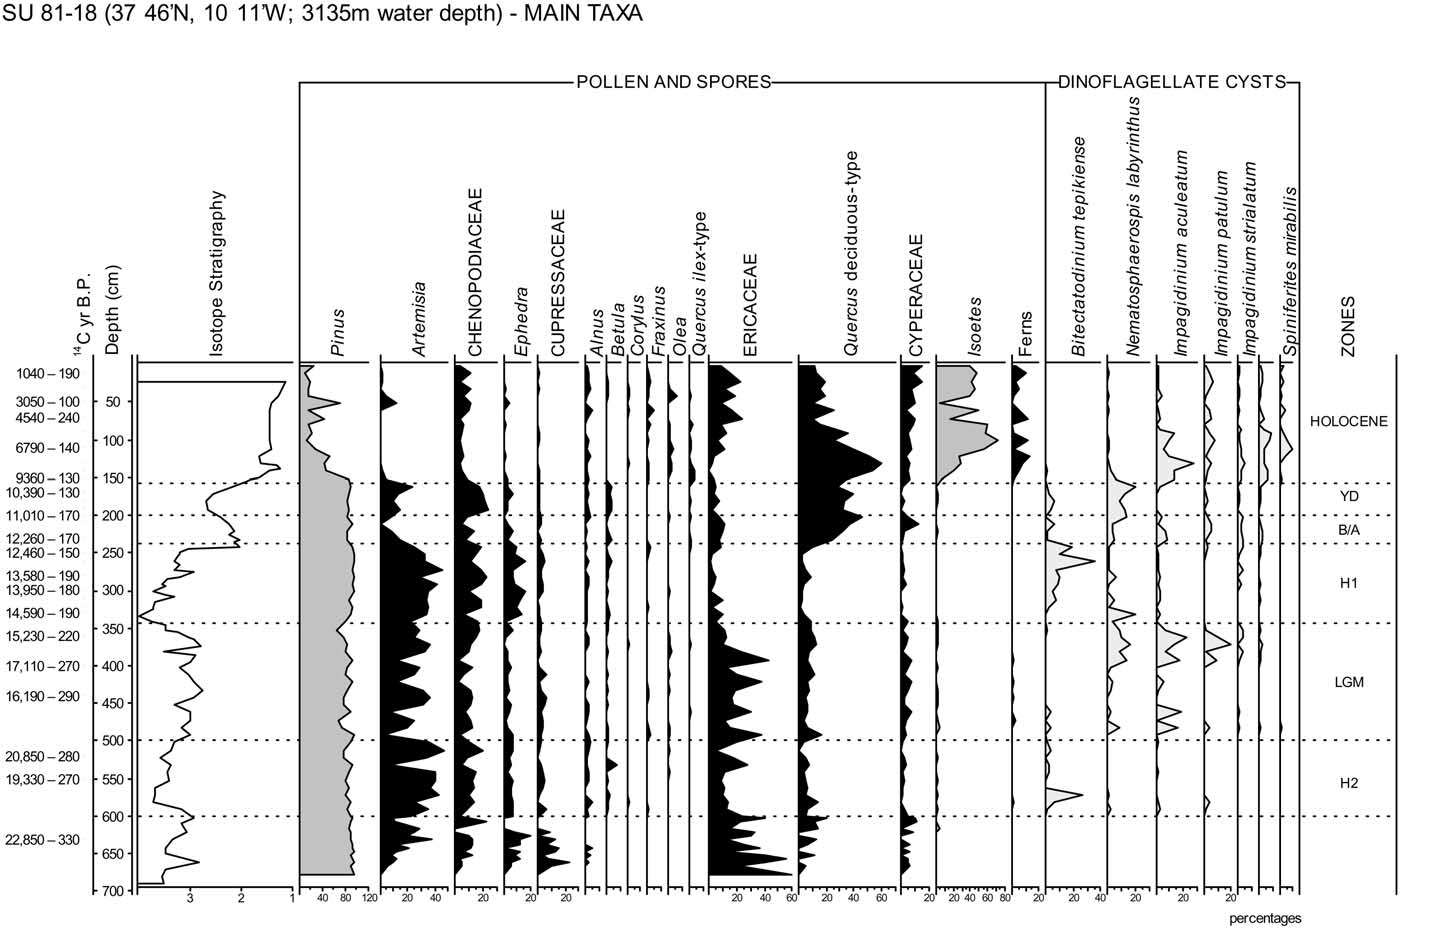
\includegraphics[width=0.8\linewidth]{figure/Turon2003_SU81-18} 

}

\caption{Diagram showing the main pollen and spore taxa and dinoflagellate cyst specimens per depth [@turon2003].}\label{fig:su8118}
\end{figure}
Faunal analysis, specifically micro-fauna, shows that these changes in habitats were followed by a change in animal incidence, with the increase of steppe adapted species, although warmer-adapted ones continued to appear in the archaeological record (Almeida, 2000). The results for mammalian fauna analysis show a dominant pattern for pronounced resilience of most animal species in the archaeological records, with a few fluctuations in the presence of wild boar, which may represent environmental responses to the rapid climate changes (Haws, 2012). Brugal and Valente (2007) also report mammalian fauna differences within the HE 2, with a broader extinction of local carnivores, while herbivore frequency remains mostly the same, with significant shifts in their spatial distribution.

Thus, despite results clearly showing that the HE 2 caused abrupt modifications in the landscape and climate of Western and Southern Iberia (Cascalheira \& Bicho, 2013), this territory still functioned as a refuge even during the colder periods (Gómez \& Lunt, 2007), in sheltered areas scattered throughout the landscape (Schmidt et al., 2012).

Although there are several paleoclimate sources which have allowed the reconstruction of the climate during the HE 2, this data cannot be fully integrated in the RRM model, to explain the emergence of the Solutrean by substitution of the Gravettian. The RRM model does not account for the Proto-Solutrean, possibly identifying it as either part of the Gravettian or Solutrean, which in a way, reflects the current understanding of the Proto-Solutrean as a transitional stage between the two technocomplexes, failing to recognize the technocomplex as an independent unit.

However, in order to fully understand the impact of the HE 2 and the environmental changes on the the replacement of the Gravettian technocomplex by the Solutrean as mentioned above, the Proto-Solutrean needs to be understood and regarded as an independent unit, as a means to understand its role in the RRM. This issue has been addressed by Cascalheira and Bicho (2013), where within the RRM, the authors suggest the Proto-Solutrean as a moment of creative destruction (Holling, 2001), which allowed the separation from the Gravettian cultural system to the development of a new structure, the Solutrean. There is, however, the need for more technological and chronological data in order to understand how the many different pieces fit together in this framework.

As such, the Proto-Solutrean stands as an essential technocomplex to understand human adaptations to climatic and environmental changes within the Upper Paleolithic.

\hypertarget{proto-solutrean-origins-and-the-portuguese-model}{%
\section{Proto-Solutrean: origins and the Portuguese model}\label{proto-solutrean-origins-and-the-portuguese-model}}

Cultural horizons within the archaeological record have been traditionally defined through the characteristics and typologies of lithic materials. The same is true for the Upper Paleolithic sequence, which in Europe was the result of several archaeological campaigns in Southwestern France, whose stratigraphic organization and sequence became the reference model across the continent (Zilhão, 1997).

Following this paradigm, the transition between the Gravettian and Solutrean was, for most of the second half of the twentieth century, based on the stratigraphy of Laugerie-Haute, in France, and thus defined in a four-stage process: Perigordian VII, Aurignacian V, Proto-Solutrean, Lower Solutrean. This succession of stages was understood as the substitution of human people and culture through processes of diffusion and migration, a paradigm present in the archaeological thought before the 1960s, and which changed drastically with the development of the New Archaeology. This new theoretical framework allowed the traditional cultural horizon sequences to be understood as the result of technological development, which did not necessarily imply the substitution of people (Zilhão, Aubry, \& Almeida, 1999). The impact of these new frameworks can be seen, for example, in the interpretation of the Perigordian VII, the first stage in the Gravettian-Solutrean transitional process. Nowadays, it is known that the Perigordian VII is, in fact, the final stage of the Gravettian (Zilhão, 1997).

The Aurignacian V, meanwhile, has been a slightly more complicated subject. Its identification was based on the presence of thick-nosed endscrapers, a technological characteristic that represented the presence of Aurignacian communities, and thus, moments of population substitution and migration in the site (Almeida, 2000; Zilhão, 1997). Part of the problem was also that this level was only known in one site in France.

The study of materials from old excavations by Manuel Heleno in Rio Maior (Portuguese Estremadura), and new archaeological works in the same region, in the 1980s, revealed assemblages from the Upper Paleolithic, some with levels of typological characteristics which parallel those of Laugerie Haute. These projects allowed one of the most comprehensive descriptions of the Upper Paleolithic occupations in Portugal, and the understanding of the Gravettian-Solutrean transition in more detail, including the problematic Aurignacian V (Almeida, 2000; Zilhão, 1994).
\begin{figure}

{\centering 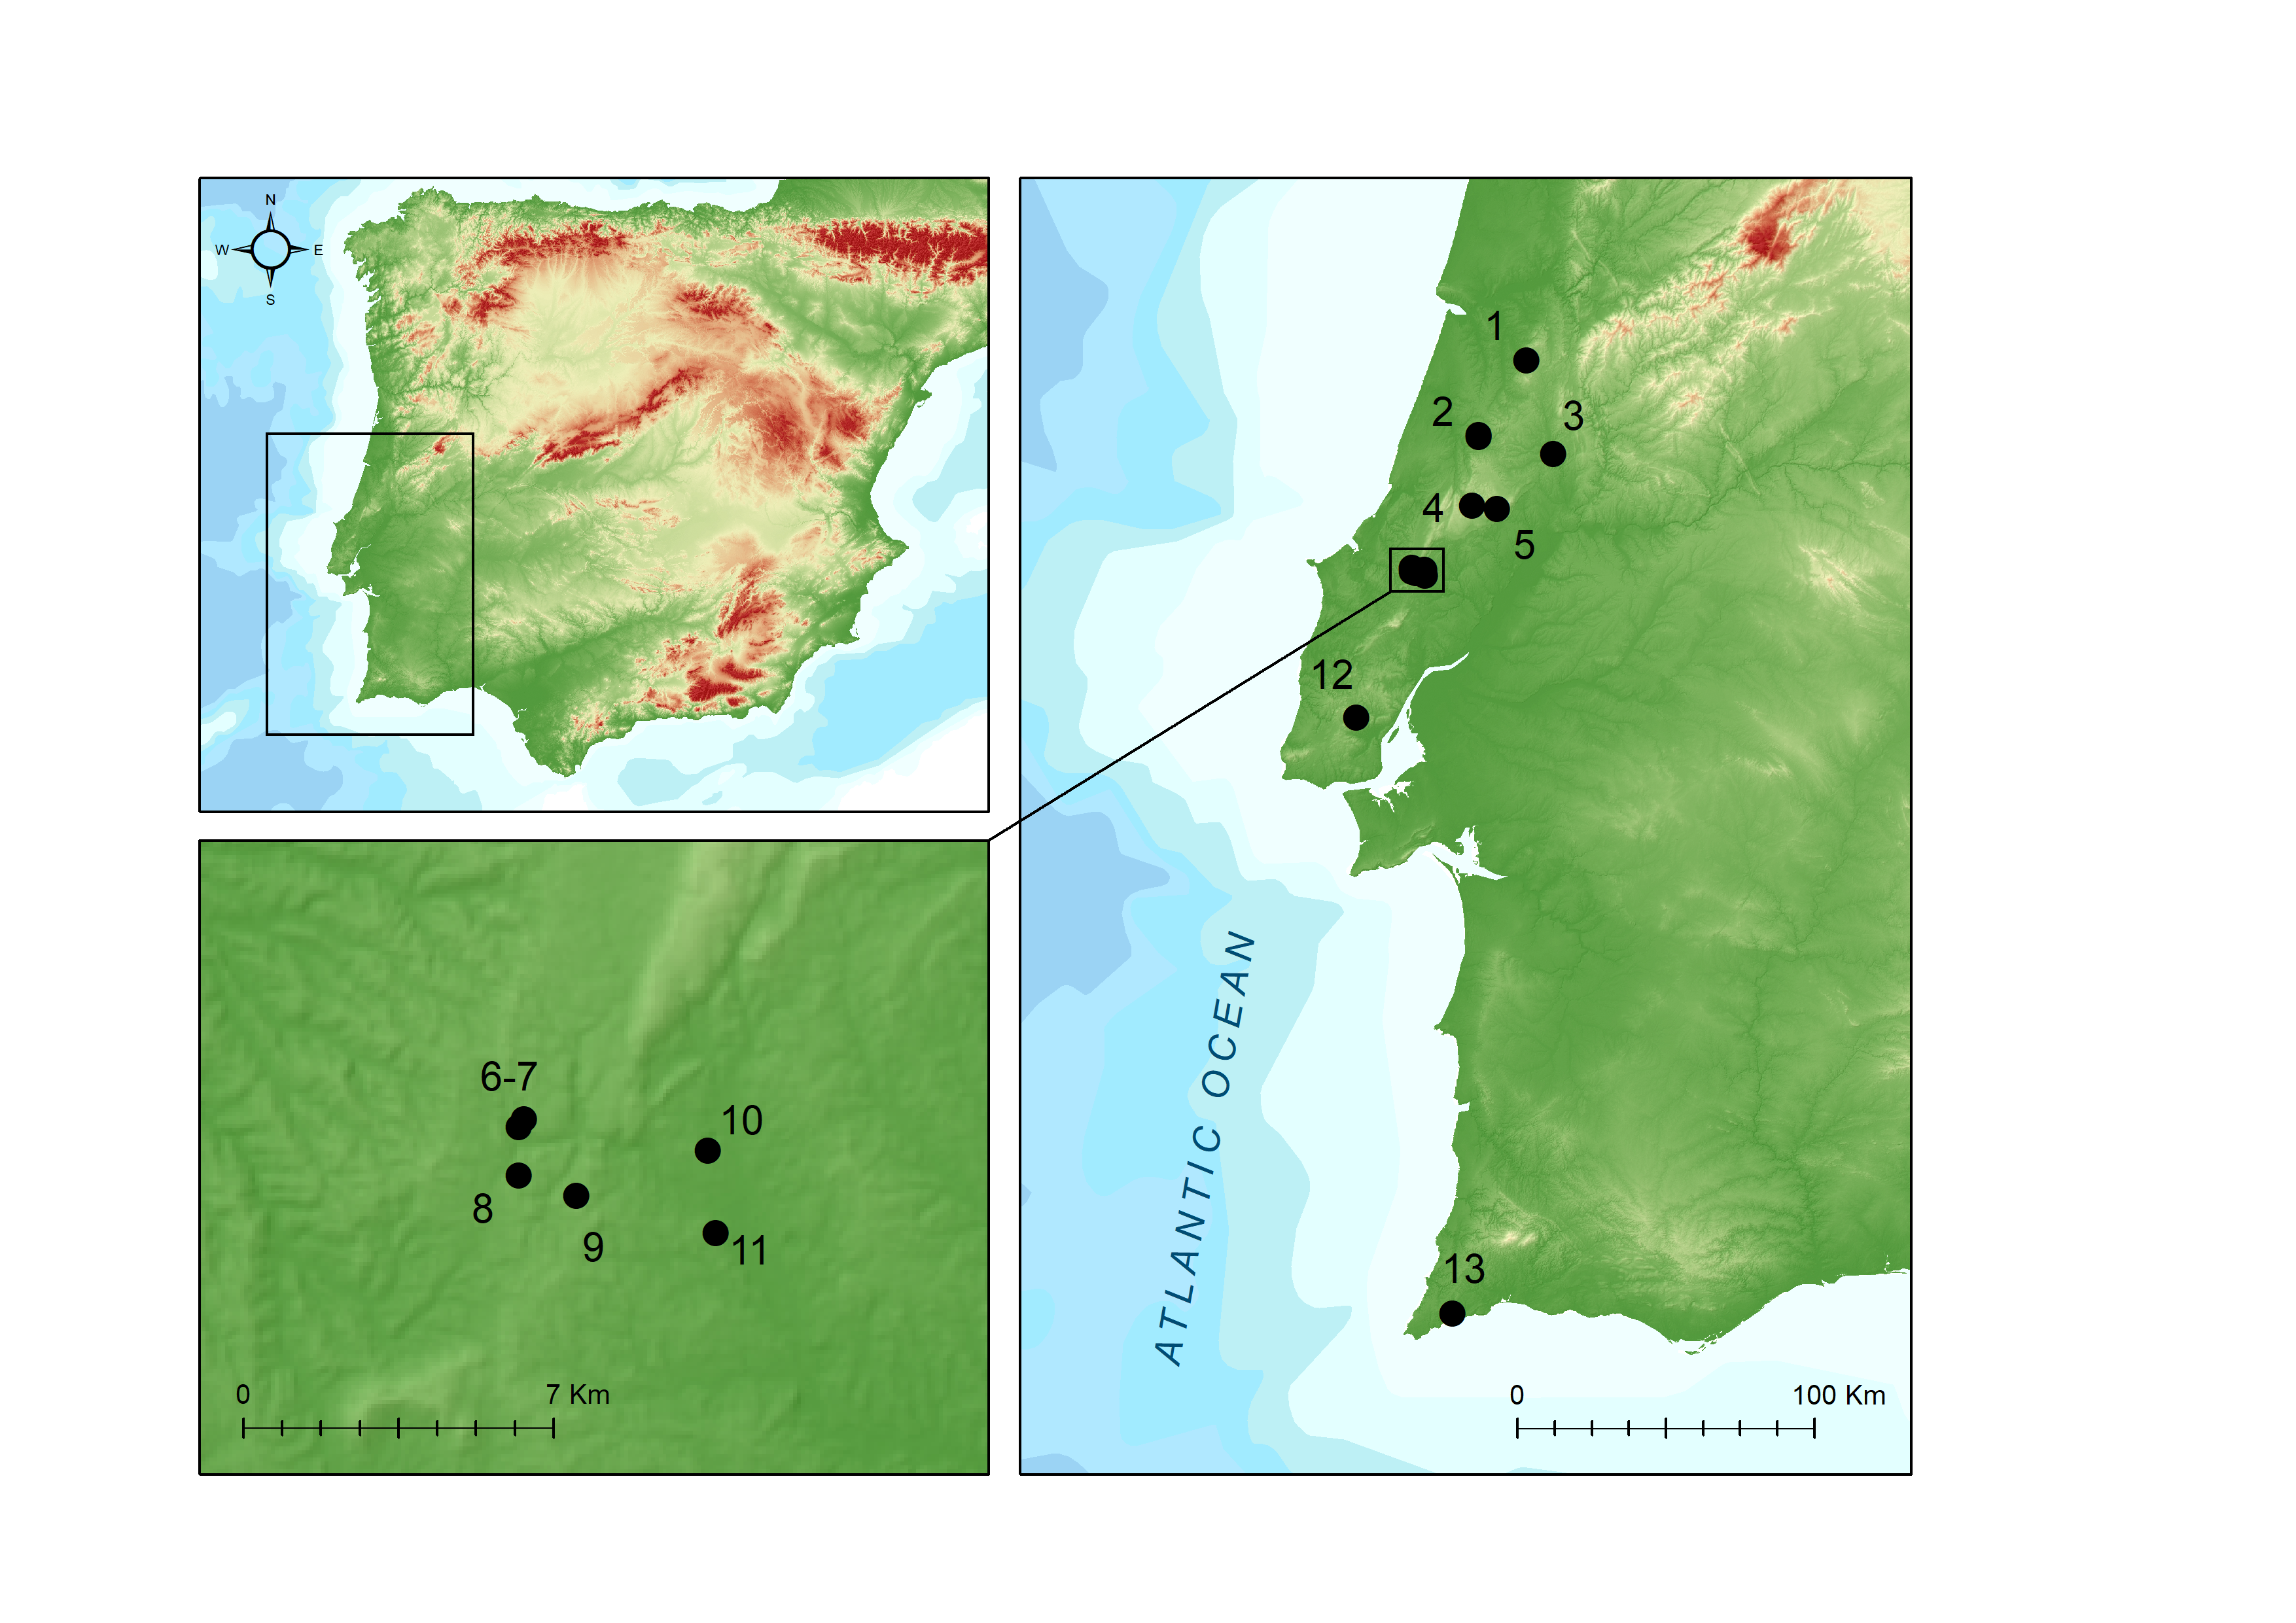
\includegraphics[width=1\linewidth]{figure/map_proto_solutrean} 

}

\caption{Location of Proto-Solutrean sites in Portugal, including the two sites analysed in this study.}\label{fig:protomap}
\end{figure}
The Proto-Solutrean has thus been described as a transitional technocomplex from Gravettian to Solutrean technologies, through a process of local development, and synchronous to all of the Southwestern Europe (Aquitaine, Pyrenees, Languedoc and the Iberian Peninsula) (Zilhão et al., 1999).

In total, 10 sites with either Proto-Solutrean assemblages or transitional characteristics were identified in the Portuguese Estremadura area (although not all have been dated, \ref{fig:protomap}). Table \ref{protodates} shows the dates for proto-solutrean occupations in Portugal, including the sites analyzed in this study.
\begin{landscape}
\begin{longtable}[t]{>{\bfseries}lllrrlrr}
\caption{\label{tab:protodates}Summary of radiocarbon dates from Portuguese Proto-Solutrean. Adapted from Zilhão (1997), Cascalheira and Bicho (2013), Belmiro (2018) and Benedetti et al. (2019). Calibration curves are IntCal13 and Marine13, using OxCal 4.1.7 (online).}\\
\toprule
Site & Level & Lab. Ref & Age (BP) & SD & Sample type & Calibrated lower 95\% & Calibrated upper 95\%\\
\midrule
\endfirsthead
\caption[]{Summary of radiocarbon dates from Portuguese Proto-Solutrean (continued).}\\
\toprule
Site & Level & Lab. Ref & Age (BP) & SD & Sample type & Calibrated lower 95\% & Calibrated upper 95\%\\
\midrule
\endhead
\
\endfoot
\bottomrule
\endlastfoot
LP & T & Wk-37655c & 18960 & 80 & Bone & 22618 & 23000\\
LP & T & UGAMS-23727 & 19530 & 50 & Charcoal & 23429 & 23639\\
LP & T & UGAMS-23718 & 20240 & 50 & Charcoal & 24199 & 24414\\
LP & T & Beta-208221e & 20240 & 110 & Charcoal & 24078 & 24543\\
LP & T & UGAMS-23725 & 20320 & 50 & Charcoal & 24295 & 24492\\
\addlinespace
Vale Boi & 5 & Wk-42831 & 20329 & 90 & Shell & 23763 & 24165\\
Alecrim & 6 & Beta-203513 & 20510 & 150 & Bone & 24331 & 25133\\
LP & T & UGAMS-23726 & 20530 & 50 & Charcoal & 24523 & 24900\\
LP & T & UGAMS-23722 & 20630 & 60 & Charcoal & 24606 & 25062\\
LP & T & Beta-229781e & 20700 & 100 & Bone & 24603 & 25217\\
\addlinespace
LP & T & UGAMS-23721 & 20710 & 60 & Charcoal & 24717 & 25163\\
Vale Boi & 5 & Wk-42830 & 20818 & 107 & Charcoal & 24724 & 25367\\
CPM III Inferior & NA & ICEN-541 & 21080 & 850 & Charcoal & 23373 & 26936\\
Lagar Velho & 6 & OxA-8420 & 21180 & 240 & Charcoal & 24879 & 25872\\
Lagar Velho & 6 & Sac-1561 & 21380 & 810 & Bone & 23839 & 27213\\
\addlinespace
Anecrial & 2b & ICEN-964 & 21560 & 680 & Charcoal & 24271 & 27249\\
Anecrial & 2b & OxA-5526 & 21560 & 220 & Charcoal & 25415 & 26208\\
Terra do Manuel & 2s & EHT-6038 & 21770 & 210 & Charcoal & 25670 & 26457\\
Alecrim & 6 & Wk-25514 & 21794 & 170 & Bone & 25775 & 26378\\
Buraca Escura & 2e & OxA-5524 & 21820 & 200 & Bone & 25755 & 26453\\
\addlinespace
Lagar Velho & 6 & OxA-8418 & 22180 & 180 & Charcoal & 26075 & 26910\\
Vale Boi & 5 & Wk-44416 & 22358 & 80 & Shell & 26018 & 26317\\
LP & U & Beta-234373e & 22560 & 110 & Charcoal & 26572 & 27150\\
LP & U & Beta-234374e & 22590 & 110 & Charcoal & 26603 & 27178\\
LP & U & Beta-208222e & 22660 & 240 & Charcoal & 26408 & 27379\\
\addlinespace
LP & T & Wk-37656 & 23100 & 130 & Charcoal & 27211 & 27591\\*
\end{longtable}
\end{landscape}
This set of dates from sites such as Anecrial, Terra do Manuel (layer 2s), Alecrim, Buraca Escura (layer 2e) and Lagar Velho (since other dates show either values which look like outliers or have extremely high standard deviations) place the transition as happening between 26.2 ka cal BP and 25.4 ka cal BP (calibrated dates from Zilhão 1997, using IntCal 13 through Oxcal online), where the lowest boundary represents the beginning of the Final Gravettian and the highest the ending of the Proto-Solutrean (Zilhão, 1997, 2000; Zilhão et al., 1999).

The understanding of the Gravettian-Solutrean transition through several phases, each with its technological characteristics and patterns, through the techno-typological characteristics of assemblages from key sites, have allowed for the creation of two models: the Two-stage model and Three-stage model (Zilhão, 1994, 1997; Zilhão et al., 1999).

The Two-stage model starts with a Final Gravettian stage, characterized by a moderate use of quartz (\textasciitilde15\%), production of truncated backed bladelets and proto-magdalenian retouch blades, where we find Terra do Manuel (old excavations and layer 2s), CPM III, CPM II and Buraca Escura (layer 2e) (Zilhão, 1997). The second stage is the Proto-Solutrean, frequently characterized by a high percentage of quartz use (\textasciitilde30\%), rare presence of backed bladelets or, when retouch is present, being marginal, and the production of Vale Comprido points, the technocomplex's index fossil (Almeida, 2000; Zilhão, 1997; ZILHÃO \& Aubry, 1995). For the production of these tools, the Proto-Solutrean shows three different operative sequences: one for the production of Vale Comprido points, through the removal of elongated blanks with convergent profiles and thick platforms; another for the production of blades, of Gravettian tradition; and another for the production of bladelets, probably obtained through the exploitation of thick endscapers or carinated elements. Proto-Solutrean phase assemblages were identified in Vale Comprido -- Encosta, Terra do José Pereira, Vales da Senhora da Luz (although Vale Comprido points are absent from the assemblage), Terra do Manuel (layer 2), Buraca Escura (layer 2b), Anecrial (layer 2) and Gato Preto (group C) (Zilhão, 1997).

Vale Comprido points are described as robust pieces, with a thickness ranging the 4-8 mm, width around 20 mm and length of about 50mm, though in some cases it may reach 80 mm, and platform thickness of 5-20 mm. They are often characterised by convergent shapes, triangular cross- sections and plain platforms, often having a high elongation ratio, although not necessarily falling into the blade category. They can also be categorized regarding retouch, with the identification of 3 groups: 1) thinning of the platform; 2) extensive retouch across the edges, including the tip; 3) an intermediate type with only partial retouch on the edges along the platform or at the tip (Zilhão, 1997; ZILHÃO \& Aubry, 1995). The Vale Comprido points have been used to describe the technological transition between the Proto-Solutrean and the Solutrean. In this case, these points are seen as an element of discontinuity with the previous technocomplex, where the organic points armed with microliths from the Gravettian are replaced by lithic points, with enough similarities to the \emph{pointes à face plane} of the Middle Solutrean to be understood as a technological development (Zilhão, 2013).

The Three-stage model maintains the first Final Gravettian stage and its defining characteristics but subdivides the following Proto-Solutrean stage in two. As such, there is an intermediate stage characterized by the intensive use of quartz (\textasciitilde30\%), which corresponds to Laugerie Haute's ``Aurignatian V'', migrating the assemblages from Terra do Manuel (layer 2s), CPM III, CPM II and Buraca Escura (layer 2b) to this phase. The third stage is the Proto-Solutrean, where quartz use diminishes. In this model, the Vale Comprido points and associated reduction sequence may appear in either of the last two stages (Zilhão, 1997). However, Almeida (2000) has noted that in the aurignacian V/terminal gravettian assemblages from the Estremadura, there seems to be the lack of Vale Comprido technology (Almeida, 2000). It may seem, thus, that this type of technology is a proto-solutrean innovation.
\begin{figure}
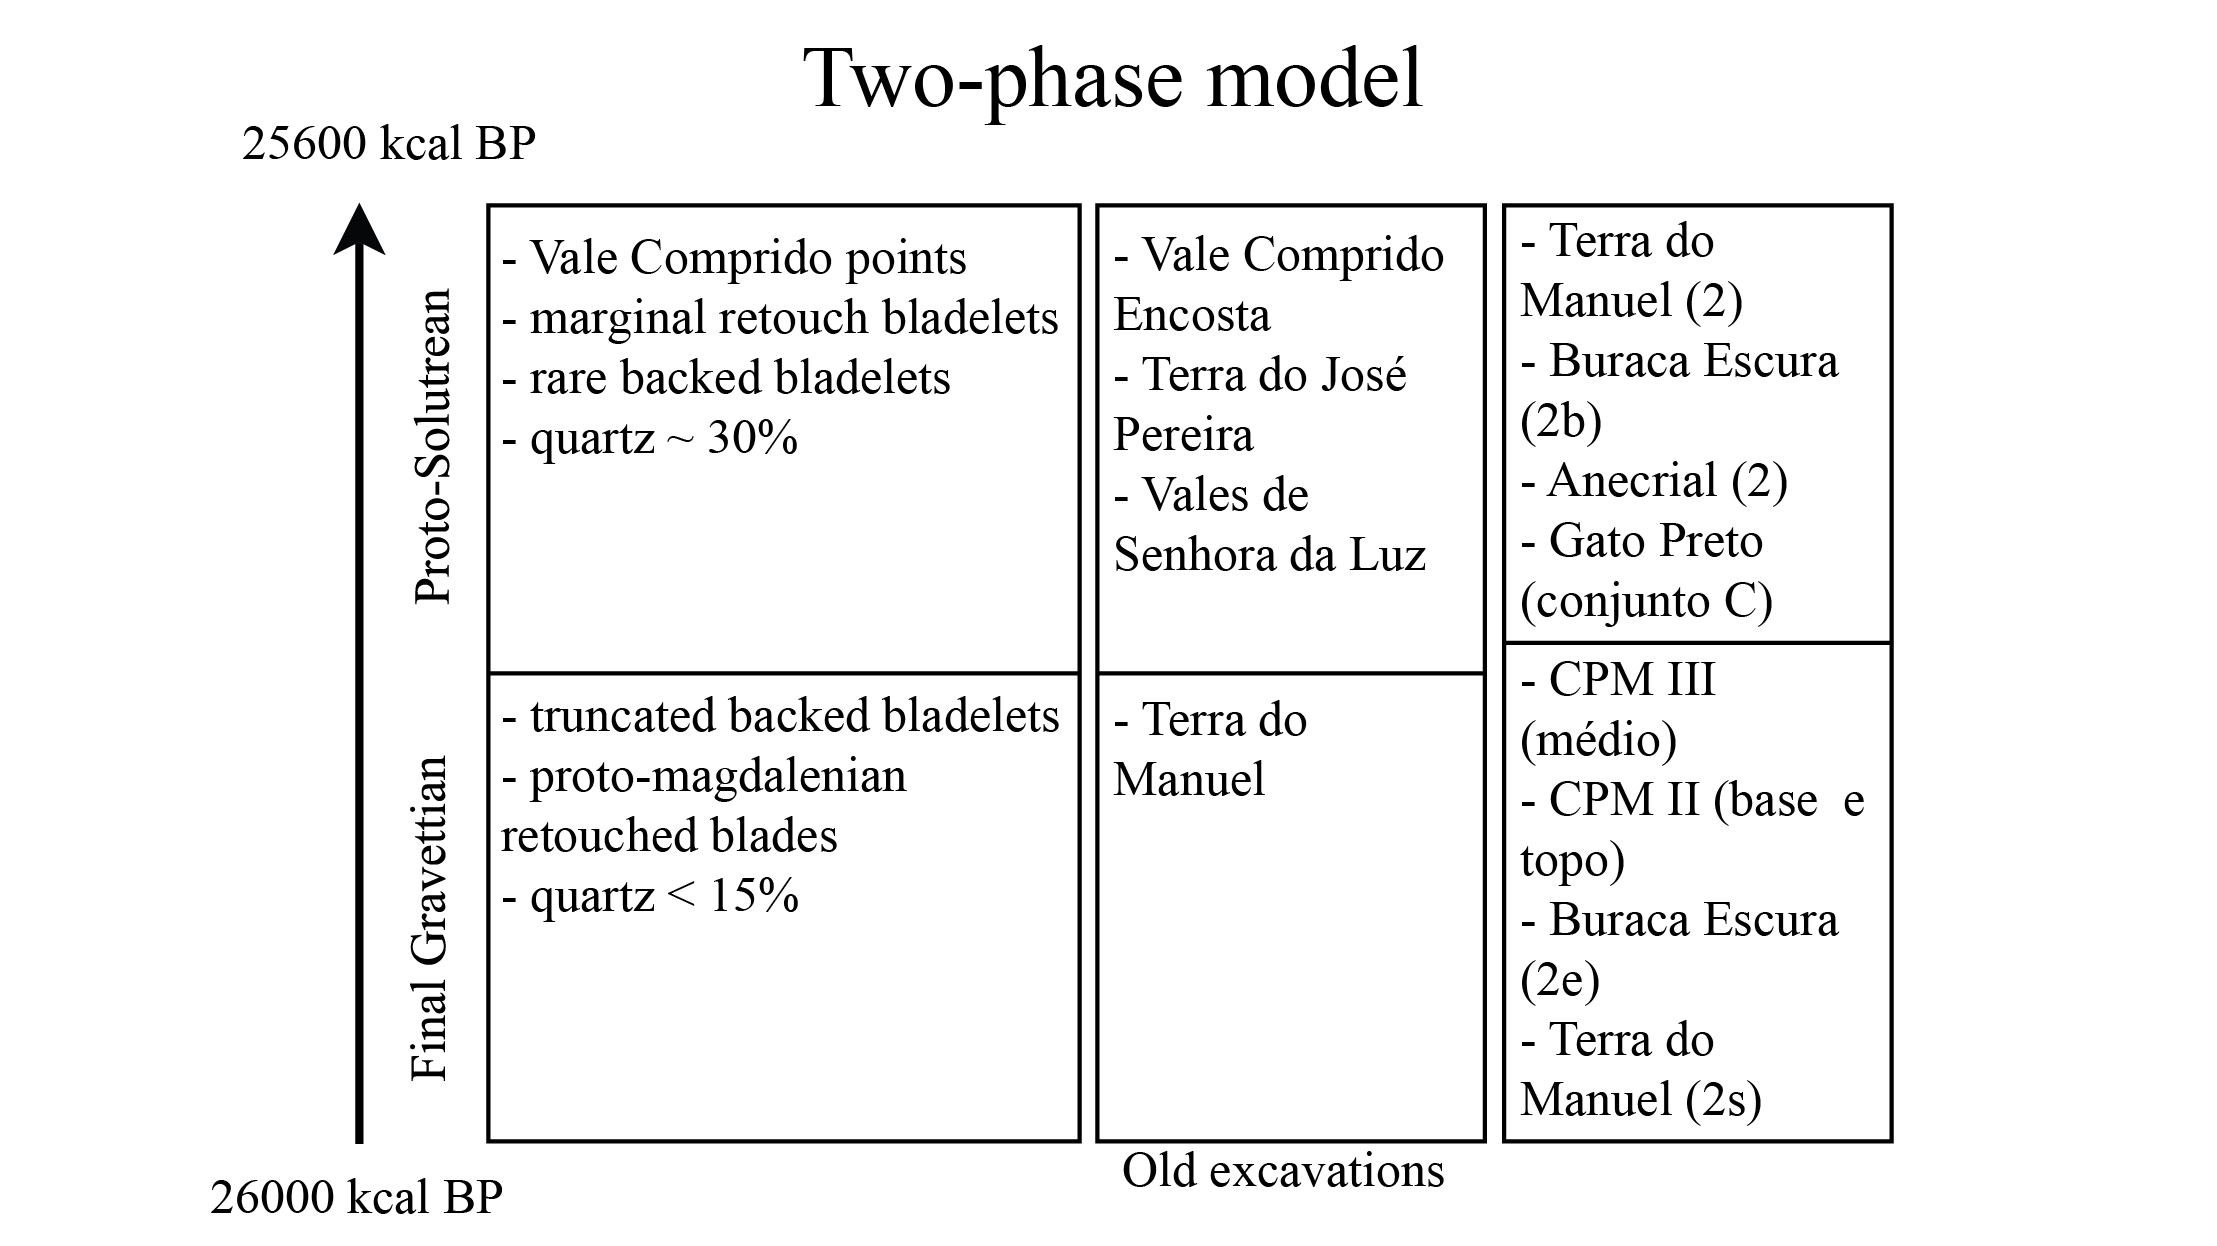
\includegraphics[width=0.8\linewidth]{figure/Two-phasemodel} \caption{Two-phase model for Gravettian to Proto-Solutrean transition, with site and archaeological level correlated with each phase. Adapted from Zilhão (1997). Model dates calibrated with curve IntCal13, using OxCal 4.1.7 (online).}\label{fig:unnamed-chunk-1}
\end{figure}
\begin{figure}
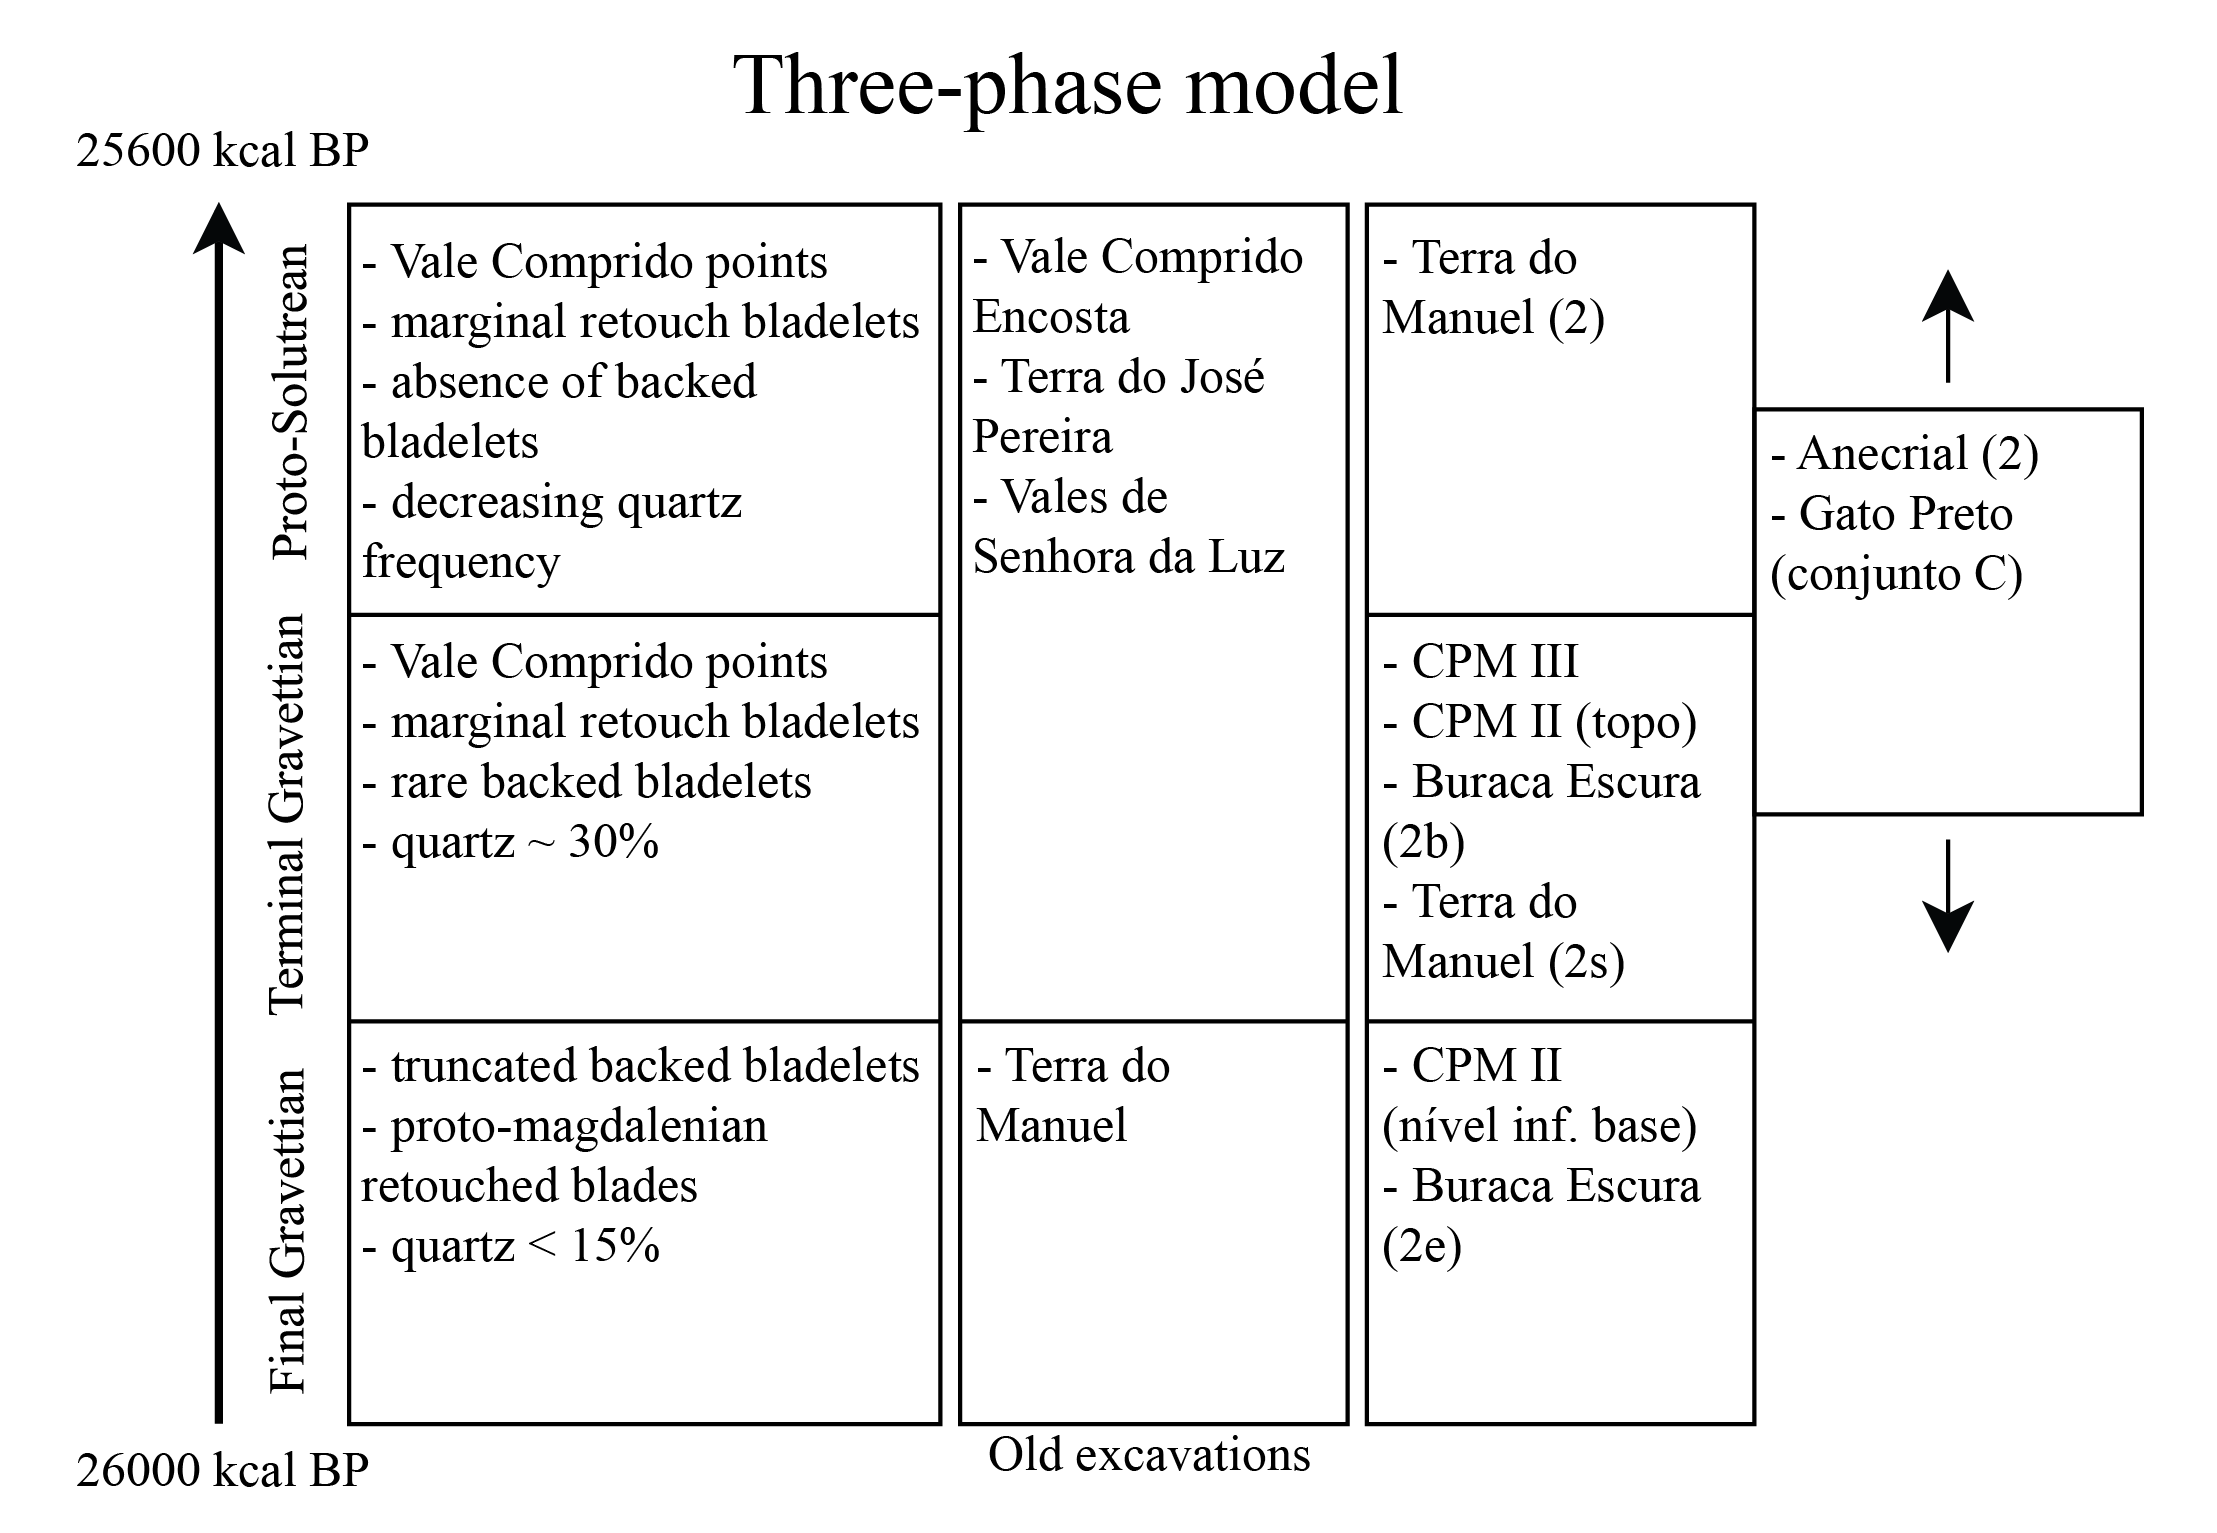
\includegraphics[width=0.8\linewidth]{figure/Three-phasemodel} \caption{Three-phase model for Gravettian to Proto-Solutrean transition, with site and archaeological level correlated with each phase. Adapted from Zilhão (1997). Model dates calibrated with curve IntCal13, using OxCal 4.1.7 (online).}\label{fig:unnamed-chunk-2}
\end{figure}
Alternatively, in the Two-phase model, the ``Aurignacian V'', is understood as a functional facies, related to specialized occupations and production activities within the technocomplex, through the observation of the coexistence of prismatic core exploitation and carinated core exploitation, both for the extraction of blades and bladelets, thus showing the latter exploitation was not an independent system as thought at Laugerie Haute (Zilhão, 1997; Zilhão et al., 1999). In fact, Zilhão (1994, 1997) has questioned the stratigraphic reality of ``Aurignacian V'' from Laugerie-Haute, interpreting it as only a typology separation due to poor stratigraphic integrity.

Almeida (2000) interprets the diagnostic Aurignacian thick-nosed endscrapers as carinated cores, with no correlation to the Aurignacian technocomplex, suggesting instead the substitution of the term Aurignacian V for Terminal Gravettian. Following previous works (Almeida, 2000; Benedetti, Haws, Bicho, Friedl, \& Ellwood, 2019; Cascalheira \& Bicho, 2013), when referring to the ``Aurignacian V'', whether as a functional facies (Two-stage model) or as an intermediate stage (Three-stage model), the present study will apply the term Terminal Gravettian instead.

One of the main differences between the models mentioned above is connected to the lithic assemblage's internal variability. In this case, the Three-stage model diminishes this internal variability by attributing chronological significance to the Terminal Gravettian (Almeida, 2000). While the Three-Phase model causes some sites to float between the Terminal Gravettian and Proto-Solutrean without an exact phase attribution (such as Terra do José Pereira, Vales da Senhora da Luz, Anecrial and Gato Preto), due to lack of necessary information or specialized character of their occupations (Zilhão, 1997), the Two-phase, because it accepts higher internal variability but also limits the number of options, guarantees that a specific phase can be attributed to all sites.

However, in the last decades, the Three-Phase model has been the most accepted, and the Terminal Gravettian phase is nowadays well-characterized technologically in Estremadura as a moment of chronological significance (Almeida, 2000), even if from a chronographic perspective, it lacks irrefutable evidence as shown by Cascalheira and Bicho (2013), for which the authors present two causes: all available radiocarbon dates, spreading through the entire HE 2 and covering the Proto-Solutrean's time-span, come from sites whose assemblages are attributed to the Terminal Gravettian (with the exception of Vale Boi); absolute ages of sites with a strong Vale Comprido component remain unknown.
Although this has been explained by some authors (e.g.~Aubry \emph{et al.}, 2011; Zilhão, 2013) as the result of strong erosive processes affecting the archaeological sites during the HE 2, other authors (Haws, 2012) fail to recognize such an extensive erosion.

Regardless of what model is accepted, the Proto-Solutrean, from the beginning of its transitional stage, stands as a technocomplex with technological innovations, reflected in the manufacture of Vale Comprido points and a complete operative sequence for their production, but marked by a high degree of technological variability in their lithic assemblages (Almeida, 2000; Zilhão, 1997; Zilhão et al., 1999).

This variability has been interpreted as a technological race in response to the environmental modifications taking course during the HE 2 (Cascalheira \& Bicho, 2013). The authors suggest that, in order to correspond to the external pressures, there may have been the need to diversify the economic strategies in use until that moment. The high exploitation of quartz, for example, formerly a secondary raw material, and the use of similar reduction strategies between quartz and chert, might represent one such economic response. The same possibly applies to the use of unprecedented raw materials for specific products, as is the case of the Proto-Solutrean levels in Vale Boi, where there is the presence of previously unknown raw materials, used mainly in the manufacture of Vale Comprido points (Belmiro, Cascalheira, \& Bicho, 2017; Marreiros, 2009). Likewise, alterations recorded in territoriality patterns for the Proto-Solutrean, which can be interpreted has extensive regional networks, may also be related to modifications in the landscape that occurred during the HE 2 (Cascalheira \& Bicho, 2013).

These technological and behavioral changes, when understood under the light of the Repeated Replacement Model previously discussed (Bradtmöller et al., 2012) and Panarchy (Holling \& Gunderson, 2002), might be understood as moments of release and restructuration led by external pressures, in this case, climate changes (Cascalheira \& Bicho, 2013).

Thus, following this framework, the Proto-Solutrean reveals itself as a moment of ``creative destruction'' (Holling, 2001), with moments of rupture and consolidation of technological innovations and social structures. In other words, the Proto-Solutrean might be understood as the moment where gravettian cultural traditions were reconfigured to best adapt to climatic and landscape alterations, setting grounds for the emergence of another phase -- the Solutrean (Cascalheira \& Bicho, 2013).

However, despite the existence of rather comprehensive literature about the technocomplex in the Portuguese Estremadura, which has allowed for a better understanding of the impacts of HE 2 in hunter-gatherer communities and the emergence of the Solutrean, there is still the need for further studies, in order to fill existing gaps. One of these gaps is the concentration of data regarding this technocomplex in the Estremadura, whereas the Proto-Solutrean is still relatively unknown in other places throughout southwestern Europe, in the case of Portugal, with only one site in the south (figure \ref{fig:protomap}). Another issue abovementioned is connected to the absence of absolute datings for Proto-Solutrean contexts, which limits the chronological definition of the technocomplex, and thus the testing of which transition model (if any) applies best (Cascalheira \& Bicho, 2013).

Addressing these issues, through the study of Proto-Solutrean lithic assemblages from other areas in the Southwestern European territory, from sites with good stratigraphic preservation which allow absolute dating and accurate spatial tracking, will undoubtedly help further understand this technocomplex, its patterns, stage transitions and possible regional variations.

\hypertarget{location-and-geological-context}{%
\chapter{Location and geological context}\label{location-and-geological-context}}

Placeholder

\hypertarget{vale-boi}{%
\section{Vale Boi}\label{vale-boi}}

\hypertarget{lapa-do-picareiro}{%
\section{Lapa do Picareiro}\label{lapa-do-picareiro}}

\hypertarget{vale-boi-1}{%
\section{Vale Boi}\label{vale-boi-1}}

\hypertarget{slope}{%
\subsection{Slope}\label{slope}}

\hypertarget{shelter}{%
\subsection{Shelter}\label{shelter}}

\hypertarget{terrace}{%
\subsection{Terrace}\label{terrace}}

\hypertarget{lapa-do-picareiro-1}{%
\section{Lapa do Picareiro}\label{lapa-do-picareiro-1}}

\hypertarget{levels-u-and-lower-t}{%
\section{Levels U and lower T}\label{levels-u-and-lower-t}}

\hypertarget{methodology}{%
\chapter{Methodology}\label{methodology}}

Placeholder

\hypertarget{attribute-analysis}{%
\section{Attribute analysis}\label{attribute-analysis}}

\hypertarget{data-analysis}{%
\section{Data analysis}\label{data-analysis}}

\hypertarget{results}{%
\chapter{Results}\label{results}}

Placeholder

\hypertarget{assemblages}{%
\section{Assemblages}\label{assemblages}}

\hypertarget{vale-boi-2}{%
\subsection{Vale Boi}\label{vale-boi-2}}

\hypertarget{lapa-do-picareiro-2}{%
\subsection{Lapa do Picareiro}\label{lapa-do-picareiro-2}}

\hypertarget{raw-materials}{%
\section{Raw materials}\label{raw-materials}}

\hypertarget{vale-boi-3}{%
\subsection{Vale Boi}\label{vale-boi-3}}

\hypertarget{quartz}{%
\subsubsection{Quartz}\label{quartz}}

\hypertarget{chert}{%
\subsubsection{Chert}\label{chert}}

\hypertarget{greywacke}{%
\subsubsection{Greywacke}\label{greywacke}}

\hypertarget{dolerite}{%
\subsubsection{Dolerite}\label{dolerite}}

\hypertarget{chalcedony}{%
\subsubsection{Chalcedony}\label{chalcedony}}

\hypertarget{lapa-do-picareiro-3}{%
\subsection{Lapa do Picareiro}\label{lapa-do-picareiro-3}}

\hypertarget{quartz-1}{%
\subsubsection{Quartz}\label{quartz-1}}

\hypertarget{chert-1}{%
\subsubsection{Chert}\label{chert-1}}

\hypertarget{technological-analysis}{%
\section{Technological analysis}\label{technological-analysis}}

\hypertarget{cores}{%
\subsection{Cores}\label{cores}}

\hypertarget{vale-boi-4}{%
\subsubsection{Vale Boi}\label{vale-boi-4}}

\hypertarget{lapa-do-picareiro-4}{%
\subsubsection{Lapa do Picareiro}\label{lapa-do-picareiro-4}}

\hypertarget{core-maintenance-products}{%
\subsection{Core maintenance products}\label{core-maintenance-products}}

\hypertarget{flakes}{%
\subsection{Flakes}\label{flakes}}

\hypertarget{vale-boi-5}{%
\subsubsection{Vale Boi}\label{vale-boi-5}}

\hypertarget{lapa-do-picareiro-5}{%
\subsubsection{Lapa do Picareiro}\label{lapa-do-picareiro-5}}

\hypertarget{elongated-blanks}{%
\subsection{Elongated blanks}\label{elongated-blanks}}

\hypertarget{vale-boi-6}{%
\subsubsection{Vale Boi}\label{vale-boi-6}}

\hypertarget{lapa-do-picareiro-6}{%
\subsubsection{Lapa do Picareiro}\label{lapa-do-picareiro-6}}

\hypertarget{retouched-tools}{%
\subsection{Retouched tools}\label{retouched-tools}}

\hypertarget{vale-boi-7}{%
\subsubsection{Vale Boi}\label{vale-boi-7}}

\hypertarget{lapa-do-picareiro-7}{%
\subsubsection{Lapa do Picareiro}\label{lapa-do-picareiro-7}}

\hypertarget{vale-comprido-technology}{%
\subsection{Vale Comprido technology}\label{vale-comprido-technology}}

\hypertarget{discussion}{%
\chapter{Discussion}\label{discussion}}

Placeholder

\hypertarget{conclusion}{%
\chapter*{Conclusion}\label{conclusion}}
\addcontentsline{toc}{chapter}{Conclusion}

Layers U/Lower T and Middle T from Lapa do Picareiro and layers 5 and 4E from Vale Boi have allowed the expansion of our understading on the Terminal Gravettian and Proto-Solutrean cultural horizons, not only testing the existing evolution models, as well as extending the geographical range of this horizon in Portugal.

As such, through the data obtained from these two sites, both recently excavated, with resource to total stations and for which a wide set of radiocarbon dates are available, the present study has reached 4 main conclusions, each responding to the goals defined in Chapter 1:
\begin{itemize}
\item
  Technological patterns are similar in the analyzed assemblages, dominated by reduction sequences focused on the obtention of elongated blanks and flakes, though prismatic cores, with little platform preparation and with resource to unidirectional strategies. These strategies are equally applied to chert and quartz.
\item
  Differences between phases within site are mostly explained by differences in raw material use and presence of Vale Comprido technology. In a first phase quartz is used in high frequencies, mainly in the production of bladelets or flakes, reducing in frequency in posterior moments. Vale Comprido technology seems to be an innovation in the second moment of occupation.
\item
  This first phase (U/Lower T and Lower 5), corresponding to a Terminal Gravettian occupation, seems to occur around 26 kcal BP. The second phase (Upper 5/4E) occurs around 25.5 kcal BP, corresponding to the Proto-Solutrean. These technological and raw material patterns correlated with the obtained dates show that the Three-phase model seems to apply best to both Estremaduran sites (as suggested by Almeida 2000) and the south of Portugal. As such, the Terminal Gravettian is not a facies, but a cultural horizon with chronological relevance.
\item
  Middle T from Lapa do Picareiro shows a horizon with technological similarities with the Proto-Solutrean, but without the diagnostic Vale Comprido technology, having instead similar blanks with some resemblances to Middle Solutrean blanks and points. Radiocarbon dates place this occupation around 24.5-24 kcal BP, which offers two hypothesis: 1) it represents a Proto-Solutrean occupation, happening at younger dates than other sites, without Vale Comprido technology; 2) it may correspond to an Early Solutrean occupation, with transitional characteristics with similarities to Proto-Solutrean and Middle Solutrean tools, a horizon yet unidentified in Portugal.
\end{itemize}
The latter is still rather inconclusive, needing further studies to understand whether there is Vale Comprido technology in Lapa do Picareiro. This may be achieved through the analysis of not only Vale Comprido technology in the Estremadura through morphological data, as well as Middle Solutrean blanks and point à face plan, without relying on typological attributes.

This may be important to understand a link that seems to be missing in the Upper Paleolithic in Portugal and that connects the Proto-Solutrean to the Middle Solutrean, further building onto the existing evolution models for the Gravettian-Solutrean transition.

Furthermore, in the future, it seems important to understand the presence of dolerite in Vale Boi. Given the now known internal characteristics of this raw material, it may be interesting to test its actual nonexistence in the other occupations in the site, to further understand possible niche expansions in this horizon, as a result to climatic changes.

\hypertarget{references}{%
\chapter*{References}\label{references}}
\addcontentsline{toc}{chapter}{References}

\markboth{References}{References}

\noindent

\setlength{\parindent}{-0.20in}
\setlength{\leftskip}{0.20in}
\setlength{\parskip}{8pt}

\hypertarget{appendix}{%
\chapter{Appendix}\label{appendix}}

Placeholder

\hypertarget{vale-boi---cores}{%
\section{VALE BOI - CORES}\label{vale-boi---cores}}

\hypertarget{vale-boi---flakes}{%
\section{VALE BOI - FLAKES}\label{vale-boi---flakes}}

\hypertarget{vale-boi---elongated}{%
\section{VALE BOI - ELONGATED}\label{vale-boi---elongated}}

\hypertarget{lapa-do-picareiro---cores}{%
\section{LAPA DO PICAREIRO - CORES}\label{lapa-do-picareiro---cores}}

\hypertarget{lapa-do-picareiro---flakes}{%
\section{LAPA DO PICAREIRO - FLAKES}\label{lapa-do-picareiro---flakes}}

\hypertarget{lapa-do-picareiro---elongated}{%
\section{LAPA DO PICAREIRO - ELONGATED}\label{lapa-do-picareiro---elongated}}

\hypertarget{refs}{}
\leavevmode\hypertarget{ref-almeida2000}{}%
Almeida, F. (2000). \emph{The terminal gravettian of portuguese estremadura. Technological variability of the lithic industries.} (PhD thesis).

\leavevmode\hypertarget{ref-belmiro2017}{}%
Belmiro, J., Cascalheira, J., \& Bicho, N. (2017). O início do último máximo glacial no sul de portugal: Novos dados a partir do sítio arqueológico de vale boi. \emph{Proceedings of the 2nd Conference of Associação Dos Arqueólogos Portugueses}.

\leavevmode\hypertarget{ref-benedettietal2019}{}%
Benedetti, M. M., Haws, J. A., Bicho, N. F., Friedl, L., \& Ellwood, B. B. (2019). Late pleistocene site formation and paleoclimate at lapa do picareiro, portugal. \emph{Geoarchaeology}, \emph{34}(6), 698--726.

\leavevmode\hypertarget{ref-bradtmoller2012}{}%
Bradtmöller, M., Pastoors, A., Weninger, B., \& Weniger, G.-C. (2012). The repeated replacement model--rapid climate change and population dynamics in late pleistocene europe. \emph{Quaternary International}, \emph{247}, 38--49.

\leavevmode\hypertarget{ref-brugal2007}{}%
Brugal, J.-P., \& Valente, M. J. (2007). Dynamic of large mammalian associations in the pleistocene of portugal. In.

\leavevmode\hypertarget{ref-cascalheira2010}{}%
Cascalheira, J. (2010). \emph{Tecnologia lítica solutrense do abrigo de vale boi (vila do bispo)}. UNIARQ.

\leavevmode\hypertarget{ref-cascalheiraandbicho2013}{}%
Cascalheira, J., \& Bicho, N. (2013). Hunter--gatherer ecodynamics and the impact of the heinrich event 2 in central and southern portugal. \emph{Quaternary International}, \emph{318}, 117--127.

\leavevmode\hypertarget{ref-fletcher2008}{}%
Fletcher, W. J., \& Goñi, M. F. S. (2008). Orbital-and sub-orbital-scale climate impacts on vegetation of the western mediterranean basin over the last 48,000 yr. \emph{Quaternary Research}, \emph{70}(3), 451--464.

\leavevmode\hypertarget{ref-gonzalez-samperiz2010}{}%
González-Sampériz, P., Leroy, S. A., Carrión, J. S., Fernández, S., García-Antón, M., Gil-García, M. J., \ldots{} Figueiral, I. (2010). Steppes, savannahs, forests and phytodiversity reservoirs during the pleistocene in the iberian peninsula. \emph{Review of Palaeobotany and Palynology}, \emph{162}(3), 427--457.

\leavevmode\hypertarget{ref-goni2000}{}%
Goñi, M. F. S., Turon, J.-L., Eynaud, F., \& Gendreau, S. (2000). European climatic response to millennial-scale changes in the atmosphere--ocean system during the last glacial period. \emph{Quaternary Research}, \emph{54}(3), 394--403.

\leavevmode\hypertarget{ref-gomez2007}{}%
Gómez, A., \& Lunt, D. H. (2007). Refugia within refugia: Patterns of phylogeographic concordance in the iberian peninsula. In \emph{Phylogeography of southern european refugia} (pp. 155--188). Springer.

\leavevmode\hypertarget{ref-haws2012}{}%
Haws, J. A. (2012). Paleolithic socionatural relationships during MIS 3 and 2 in central portugal. \emph{Quaternary International}, \emph{264}, 61--77.

\leavevmode\hypertarget{ref-heinrich1988}{}%
Heinrich, H. (1988). Origin and consequences of cyclic ice rafting in the northeast atlantic ocean during the past 130,000 years. \emph{Quaternary Research}, \emph{29}(2), 142--152.

\leavevmode\hypertarget{ref-holling2001}{}%
Holling, C. S. (2001). Understanding the complexity of economic, ecological, and social systems. \emph{Ecosystems}, \emph{4}(5), 390--405.

\leavevmode\hypertarget{ref-holling2002}{}%
Holling, C. S., \& Gunderson, L. H. (2002). \emph{Panarchy: Understanding transformations in human and natural systems}. Washington, DC: Island Press.

\leavevmode\hypertarget{ref-holst2017}{}%
Holst, M. J. (2017). Late magdalenian lithic technological organization at lapa do picareiro, central portugal.

\leavevmode\hypertarget{ref-marreiros2009}{}%
Marreiros, J. M. F. (2009). \emph{As primeiras comunidades do homem moderno no algarve ocidental: Caracterização paleotecnológica e paleoetnográfica das comunidades gravetenses e proto-solutrenses de vale boi (algarve, portugal)} (PhD thesis).

\leavevmode\hypertarget{ref-naughton2007}{}%
Naughton, F., Goñi, M. S., Desprat, S., Turon, J.-L., Duprat, J., Malaizé, B., \ldots{} Freitas, M. C. (2007). Present-day and past (last 25 000 years) marine pollen signal off western iberia. \emph{Marine Micropaleontology}, \emph{62}(2), 91--114.

\leavevmode\hypertarget{ref-roche1971}{}%
Roche, J. (1971). \emph{Le climat et les faunes du paléolithique moyen et supérieur de la province d'Estremadura}.

\leavevmode\hypertarget{ref-roche1977}{}%
Roche, J. (1977). QUELQUES INDICATIONS SUR LE MILIEU DE LA PROVINCE d'ESTREMODURA (PORTUGAL) AU PLEISTOCENE FINAL.

\leavevmode\hypertarget{ref-sanchez-goni2010}{}%
Sanchez Goñi, M. F., \& Harrison, S. P. (2010). Millennial-scale climate variability and vegetation changes during the last glacial: Concepts and terminology. \emph{Quaternary Science Reviews}, \emph{29}(21), 2823--2827.

\leavevmode\hypertarget{ref-schmidt2012}{}%
Schmidt, I., Bradtmöller, M., Kehl, M., Pastoors, A., Tafelmaier, Y., Weninger, B., \& Weniger, G.-C. (2012). Rapid climate change and variability of settlement patterns in iberia during the late pleistocene. \emph{Quaternary International}, \emph{274}, 179--204.

\leavevmode\hypertarget{ref-thacker1996}{}%
Thacker, P. T. (1996). Hunter-gatherer lithic economy and settlement systems. In \emph{Stone tools} (pp. 101--124). Springer.

\leavevmode\hypertarget{ref-turon2003}{}%
Turon, J.-L., Lézine, A.-M., \& Denèfle, M. (2003). Land--sea correlations for the last glaciation inferred from a pollen and dinocyst record from the portuguese margin. \emph{Quaternary Research}, \emph{59}(1), 88--96.

\leavevmode\hypertarget{ref-zilhao1994}{}%
Zilhão, J. (1994). La séquence chrono--stratigraphique du solutréen portugais. \emph{Férvedes}, \emph{1}, 119--129.

\leavevmode\hypertarget{ref-zilhao1997}{}%
Zilhão, J. (1997). \emph{O paleolítico superior da estremadura portuguesa, volume i}.

\leavevmode\hypertarget{ref-zilhao2000}{}%
Zilhão, J. (2000). Nature and culture in portugal from 30,000 to 20,000 BP. \emph{Hunters of the Golden Age: The Mid-Upper Paleolithic of Eurasia}, \emph{30}, 337--354.

\leavevmode\hypertarget{ref-zilhao2013}{}%
Zilhão, J. (2013). Seeing the leaves and not missing the forest: A portuguese perspective of the solutrean. \emph{Pleistocene Foragers on the Iberian Peninsula: Their Culture and Environment. Festschrift in Honour of Gerd-Christian Weniger for His Sixtieth Birthday}, 201--2016.

\leavevmode\hypertarget{ref-zilhaoetal1995}{}%
ZILHÃO, J., \& Aubry, T. (1995). La pointe de vale comprido et les origines du solutréen. \emph{L'Anthropologie}, \emph{99}(1), 125--142.

\leavevmode\hypertarget{ref-zilhaoetal1999}{}%
Zilhão, J., Aubry, T., \& Almeida, F. (1999). Un modèle technologique pour le passage du gravettien au solutréen dans le sud-ouest de l'Europe. \emph{Les Faciès Leptolithiques Du Nord-Ouest Méditerranéen: Milieux Naturels et Culturels. Actes Du XXIVe Congrès Préhistorique de France (Carcassonne 1994)}, 165--183.


% Index?

\end{document}
